\section{Thuật toán Apostolico-Crochemore}

\subsection{Đặc điểm chính}

Thuật toán Apostolico–Crochemore là một thuật toán tìm kiếm mẫu trong chuỗi, được thiết kế nhằm cải thiện hiệu quả so với các 
phương pháp kinh điển như Brute Force và các thuật toán dựa trên tiền xử lý đơn thuần. 
Ý tưởng chính của thuật toán là kết hợp giữa tiền xử lý mẫu và việc tận dụng thông tin đã thu được trong quá trình quét văn bản, từ đó giảm số lần so sánh ký tự không cần thiết và tối ưu hóa bước dịch cửa sổ tìm kiếm.

Thuật toán thực hiện so sánh ký tự theo hướng từ trái sang phải và đạt hiệu quả cao nhờ cơ chế tránh quay lui trên văn bản. 
Pha tiền xử lý và pha tìm kiếm đều được tối ưu để đảm bảo hiệu năng tuyến tính, 
đồng thời hạn chế tối đa số phép so sánh dư thừa trong quá trình xử lý chuỗi. Cụ thể, thuật toán có các đặc điểm sau:

\begin{itemize}
    \item pha tiền xử lý có độ phức tạp thời gian và không gian $O(m)$;
    \item pha tìm kiếm có độ phức tạp thời gian $O(n)$;
    \item trong trường hợp xấu nhất, số phép so sánh ký tự trên văn bản bị chặn bởi $\frac{3}{2}n$.
\end{itemize}

\subsection{Mô tả thuật toán}

Thuật toán Apostolico–Crochemore sử dụng bảng dịch \texttt{kmpNext} (xem Chương 3.3, thuật toán Knuth–Morris–Pratt) 
để tính các bước dịch.

Gọi $\ell = 0$ nếu $x$ là một lũy thừa của một ký tự đơn (tức là $x = c^m$ với $c \in \Sigma$), và $\ell$ 
bằng vị trí của ký tự đầu tiên trong $x$ khác với $x[0]$ 
trong trường hợp còn lại (tức là $x = a^\ell bu$, với $a, b \in \Sigma$, $u \in \Sigma^*$ và $a \neq b$).

Trong mỗi lần thử, các phép so sánh được thực hiện theo thứ tự các vị trí trong mẫu như sau:
\[
\ell, \ell+1, \ldots, m-2, m-1, 0, 1, \ldots, \ell-1.
\]

Trong pha tìm kiếm, ta xét các bộ ba có dạng $(i, j, k)$ trong đó:
\begin{itemize}
    \item cửa sổ đang được đặt tại đoạn văn bản $y[j \dots j+m-1]$;
    \item $0 \leq k \leq \ell$ và $x[0 \dots k-1] = y[j \dots j+k-1]$;
    \item $\ell \leq i < m$ và $x[\ell \dots i-1] = y[j+\ell \dots j+i-1]$.
\end{itemize}

Bộ ba khởi đầu là $(\ell, 0, 0)$.

\begin{figure}[H]
    \centering
    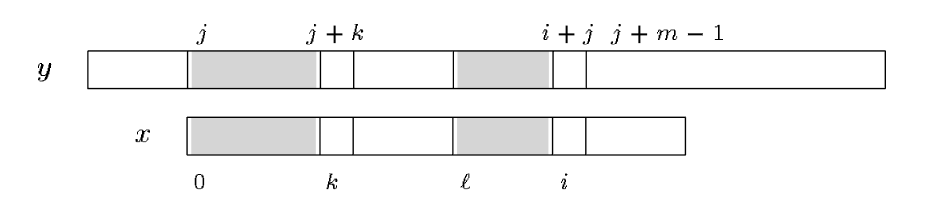
\includegraphics[width=10cm]{Images/2026-05-15-10-31-03.png}
    \caption{Minh họa bộ ba (i, j, k) trong thuật toán Apostolico-Crochemore}
    \label{fig:apostolico-crochemore-triple}
\end{figure}

Bây giờ ta giải thích cách tính bộ ba tiếp theo sau khi bộ ba $(i, j, k)$ đã được tính. 
Ba trường hợp phát sinh tùy theo giá trị của $i$:

\begin{description}

\item[Trường hợp $i = \ell$:] \hfill\\

\begin{itemize}
  \item Nếu $x[i] = y[i+j]$ thì bộ ba tiếp theo là $(i+1,\, j,\, k)$.
  \item Nếu $x[i] \neq y[i+j]$ thì bộ ba tiếp theo là
        $(\ell,\, j+1,\, \max\{0,\, k-1\})$.
\end{itemize}

\item[Trường hợp $\ell < i < m$:] \hfill\\
\begin{itemize}
  \item Nếu $x[i] = y[i+j]$ thì bộ ba tiếp theo là $(i+1,\, j,\, k)$.
  \item Nếu $x[i] \neq y[i+j]$ thì lại có hai trường hợp con tùy theo
        giá trị của $\mathit{kmpNext}[i]$:
        \begin{itemize}
          \item $\mathit{kmpNext}[i] \leq \ell$: bộ ba tiếp theo là
                $\bigl(\ell,\; i+j-\mathit{kmpNext}[i],\;
                \max\{0,\,\mathit{kmpNext}[i]\}\bigr)$.
          \item $\mathit{kmpNext}[i] > \ell$: bộ ba tiếp theo là
                $\bigl(\mathit{kmpNext}[i],\; i+j-\mathit{kmpNext}[i],\;
                \ell\bigr)$.
        \end{itemize}
\end{itemize}

\item[Trường hợp $i = m$:] \hfill\\

\begin{itemize}
    \item Nếu $k < \ell$ và $x[k] = y[j+k]$ thì bộ ba tiếp theo là $(i,\, j,\, k+1)$.
    \item Ngược lại --- hoặc $k < \ell$ và $x[k] \neq y[j+k]$, hoặc $k = \ell$. Nếu $k = \ell$, 
    một lần xuất hiện của $x$ được ghi nhận. 
    Trong cả hai trường hợp này, bộ ba tiếp theo được tính theo cách tương tự như trường hợp $\ell < i < m$.
\end{itemize}


\end{description}

Pha tiền xử lý bao gồm việc tính bảng $\mathit{kmpNext}$ và số nguyên $\ell$.
Pha này có thể thực hiện trong $O(m)$ không gian và thời gian.
Pha tìm kiếm có độ phức tạp thời gian $O(n)$; hơn nữa, thuật toán
Apostolico--Crochemore thực hiện nhiều nhất $\frac{3}{2}n$ phép so sánh
ký tự văn bản trong trường hợp xấu nhất.

\subsection{Cài đặt bằng C++}
\begin{verbatim}
#include <vector>
#include <string>
#include <algorithm>
#include <functional>

void preKmp(const std::string& x, int m, std::vector<int>& kmpNext) {
    int i = 0, j = kmpNext[0] = -1;
    while (i < m) {
        while (j > -1 && x[i] != x[j])
            j = kmpNext[j];
        kmpNext[++i] = ++j;
        if (x[i] == x[j])
            kmpNext[i] = kmpNext[j];
    }
}

std::vector<int> AXAMAC(const std::string& x, const std::string& y) {
    int m = static_cast<int>(x.size());
    int n = static_cast<int>(y.size());
    std::vector<int> kmpNext(m + 1);
    std::vector<int> results;

    /* Preprocessing */
    preKmp(x, m, kmpNext);
    int ell = 1;
    while (ell < m && x[ell - 1] == x[ell])
        ++ell;
    if (ell == m)
        ell = 0;

    /* Searching */
    int i = ell, j = 0, k = 0;
    while (j <= n - m) {
        while (i < m && x[i] == y[i + j])
            ++i;
        if (i >= m) {
            while (k < ell && x[k] == y[j + k])
                ++k;
            if (k >= ell)
                results.push_back(j); // OUTPUT(j)
        }
        j += (i - kmpNext[i]);
        if (i == ell) {
            k = std::max(0, k - 1);
        } else if (kmpNext[i] <= ell) {
            k = std::max(0, kmpNext[i]);
            i = ell;
        } else {
            k = ell;
            i = kmpNext[i];
        }
    }

    return results;
}
\end{verbatim}

\subsection{Kiểm nghiệm thuật toán}

\begin{figure}[H]
    \centering
    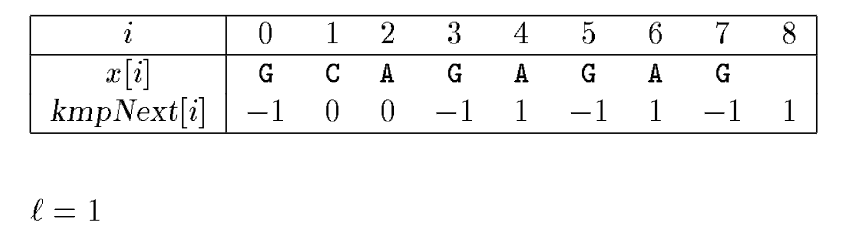
\includegraphics[width=10cm]{Images/2026-05-15-10-42-19.png}
    \caption{Kết quả kiểm nghiệm thuật toán Apostolico-Crochemore}
    \label{fig:apostolico-crochemore-test-overview}
\end{figure}

\textbf{Pha tìm kiếm}

Lần 1:

\begin{figure}[H]
    \centering
    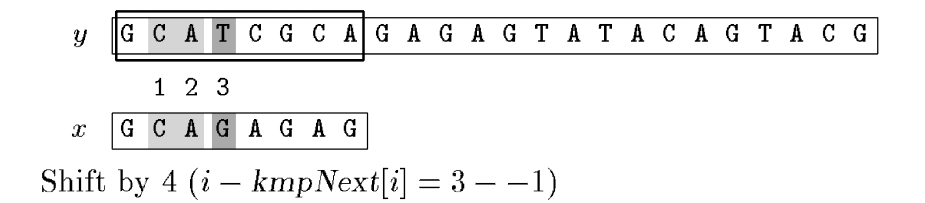
\includegraphics[width=10cm]{Images/2026-05-15-10-43-59.png}
    \caption{Bước 1 trong quá trình thực hiện thuật toán Apostolico-Crochemore}
    \label{fig:apostolico-crochemore-step-1}
\end{figure}


Lần 2:

\begin{figure}[H]
    \centering
    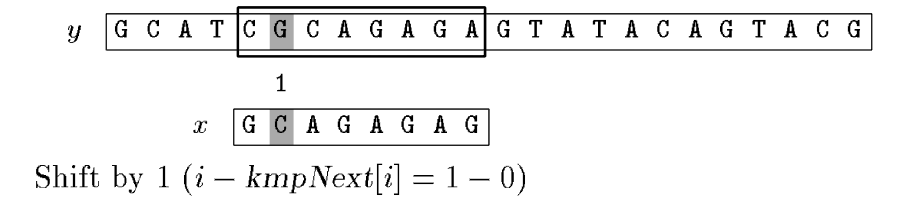
\includegraphics[width=10cm]{Images/2026-05-15-10-44-13.png}
    \caption{Bước 2 trong quá trình thực hiện thuật toán Apostolico-Crochemore}
    \label{fig:apostolico-crochemore-step-2}
\end{figure}


Lần 3:

\begin{figure}[H]
    \centering
    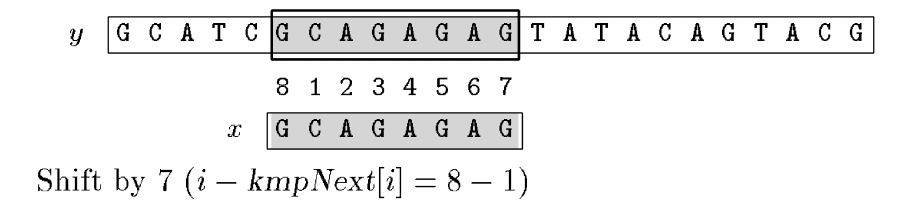
\includegraphics[width=10cm]{Images/2026-05-15-10-44-25.png}
    \caption{Bước 3 trong quá trình thực hiện thuật toán Apostolico-Crochemore}
    \label{fig:apostolico-crochemore-step-3}
\end{figure}


Lần 4:

\begin{figure}[H]
    \centering
    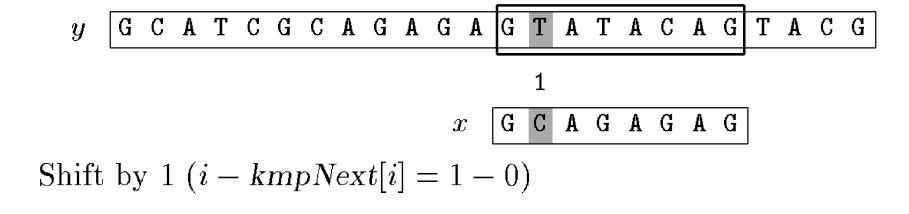
\includegraphics[width=10cm]{Images/2026-05-15-10-44-36.png}
    \caption{Bước 4 trong quá trình thực hiện thuật toán Apostolico-Crochemore}
    \label{fig:apostolico-crochemore-step-4}
\end{figure}

Lần 5:

\begin{figure}[H]
    \centering
    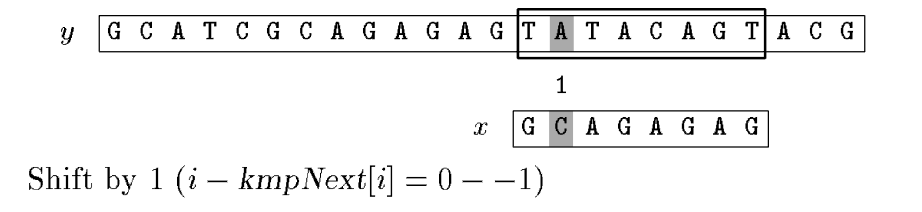
\includegraphics[width=10cm]{Images/2026-05-15-10-44-49.png}
    \caption{Bước 5 trong quá trình thực hiện thuật toán Apostolico-Crochemore}
    \label{fig:apostolico-crochemore-step-5}
\end{figure}

Lần 6:

\begin{figure}[H]
    \centering
    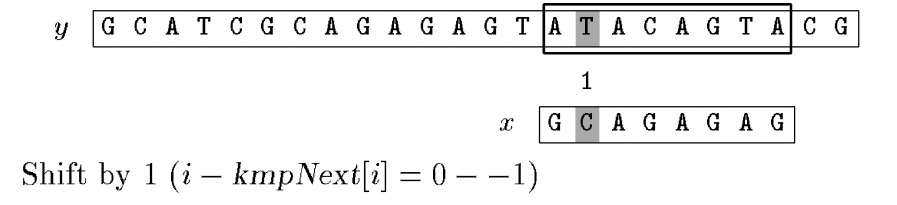
\includegraphics[width=10cm]{Images/2026-05-15-10-44-59.png}
    \caption{Bước 6 trong quá trình thực hiện thuật toán Apostolico-Crochemore}
    \label{fig:apostolico-crochemore-step-6}
\end{figure}

Lần 7:

\begin{figure}[H]
    \centering
    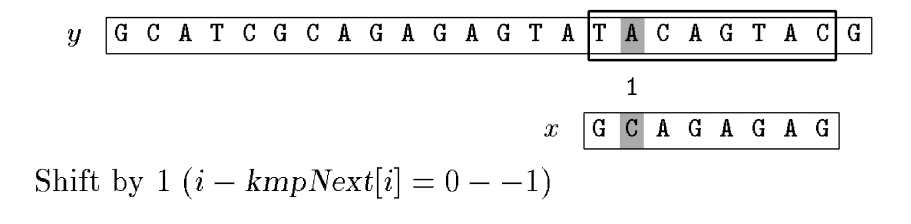
\includegraphics[width=10cm]{Images/2026-05-15-10-45-08.png}
    \caption{Bước 7 trong quá trình thực hiện thuật toán Apostolico-Crochemore}
    \label{fig:apostolico-crochemore-step-7}
\end{figure}

Lần 8:

\begin{figure}[H]
    \centering
    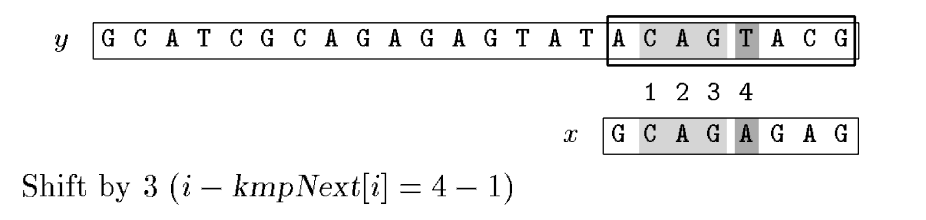
\includegraphics[width=10cm]{Images/2026-05-15-10-45-53.png}
    \caption{Bước 8 trong quá trình thực hiện thuật toán Apostolico-Crochemore}
    \label{fig:apostolico-crochemore-step-8}
\end{figure}

Trong ví dụ trên, thuật toán Apostolico-Crochemore thực hiện 20 lần so sánh chuỗi.